\documentclass[11pt, a4paper]{report}

\usepackage[T1]{fontenc}
\usepackage[utf8]{inputenc} 
\usepackage[english]{babel}
\usepackage[top=3cm, bottom=3cm, left=2cm, right=2cm]{geometry}
\usepackage{graphics}
\usepackage{graphicx}
\usepackage{eurosym}
\usepackage{soul}
\usepackage{graphicx} %utilisation d'images
\usepackage{amsmath}
\usepackage{relsize}
\usepackage{titlepic}


\begin{titlepage}
\newcommand*{\defeq}{\stackrel{\mathsmaller{\mathsf{def}}}{=}}
\title{Devoir de conception UML :\\Application de gestion des stages}
\author{GARCIA  Guillaume et ZAMBAUX Gauthier}
\date{\today}
\titlepic{
\includegraphics[scale=0.5]{Images/telecomnancy.png}

\includegraphics[scale=1]{Images/universitelorraine.jpg}}
\end{titlepage}



\begin{document}
\maketitle


\chapter*{Introduction}
\hspace{1cm}Ce devoir consiste en la complétion du cahier des charges déjà présenté qui visait à définir les règles de création d’une application de gestion des stages des élèves de TELECOM Nancy. Il nous a ainsi été demandé de préciser le fonctionnement d’un certain nombre de fonctionnalités de l’application.\vspace{0.2cm}

\hspace{0.6cm}Dans ce rapport, nous présentons à la suite un diagramme de classes venant compléter le diagramme entités-associations déjà présenté dans le SRS et qui peut être trouvé en annexe de ce devoir, trois diagrammes de séquence et le diagramme d’états d’une demande de stage.\vspace{0.2cm}

\hspace{0.6cm}Les trois diagrammes de séquence correspondent dans l’ordre à la saisie de la fiche de renseignements, à la prise de décision concernant cette même fiche et à l’initialisation d’une nouvelle année.\vspace{0.2cm}

\hspace{0.6cm}Nous avons, pour la création des diagrammes, utilisé le logiciel PlantUML (plantuml.com). Les codes UML des différents diagrammes peuvent par ailleurs être trouvés en annexe de ce rapport.

\chapter*{Diagramme des classes}
\centerline{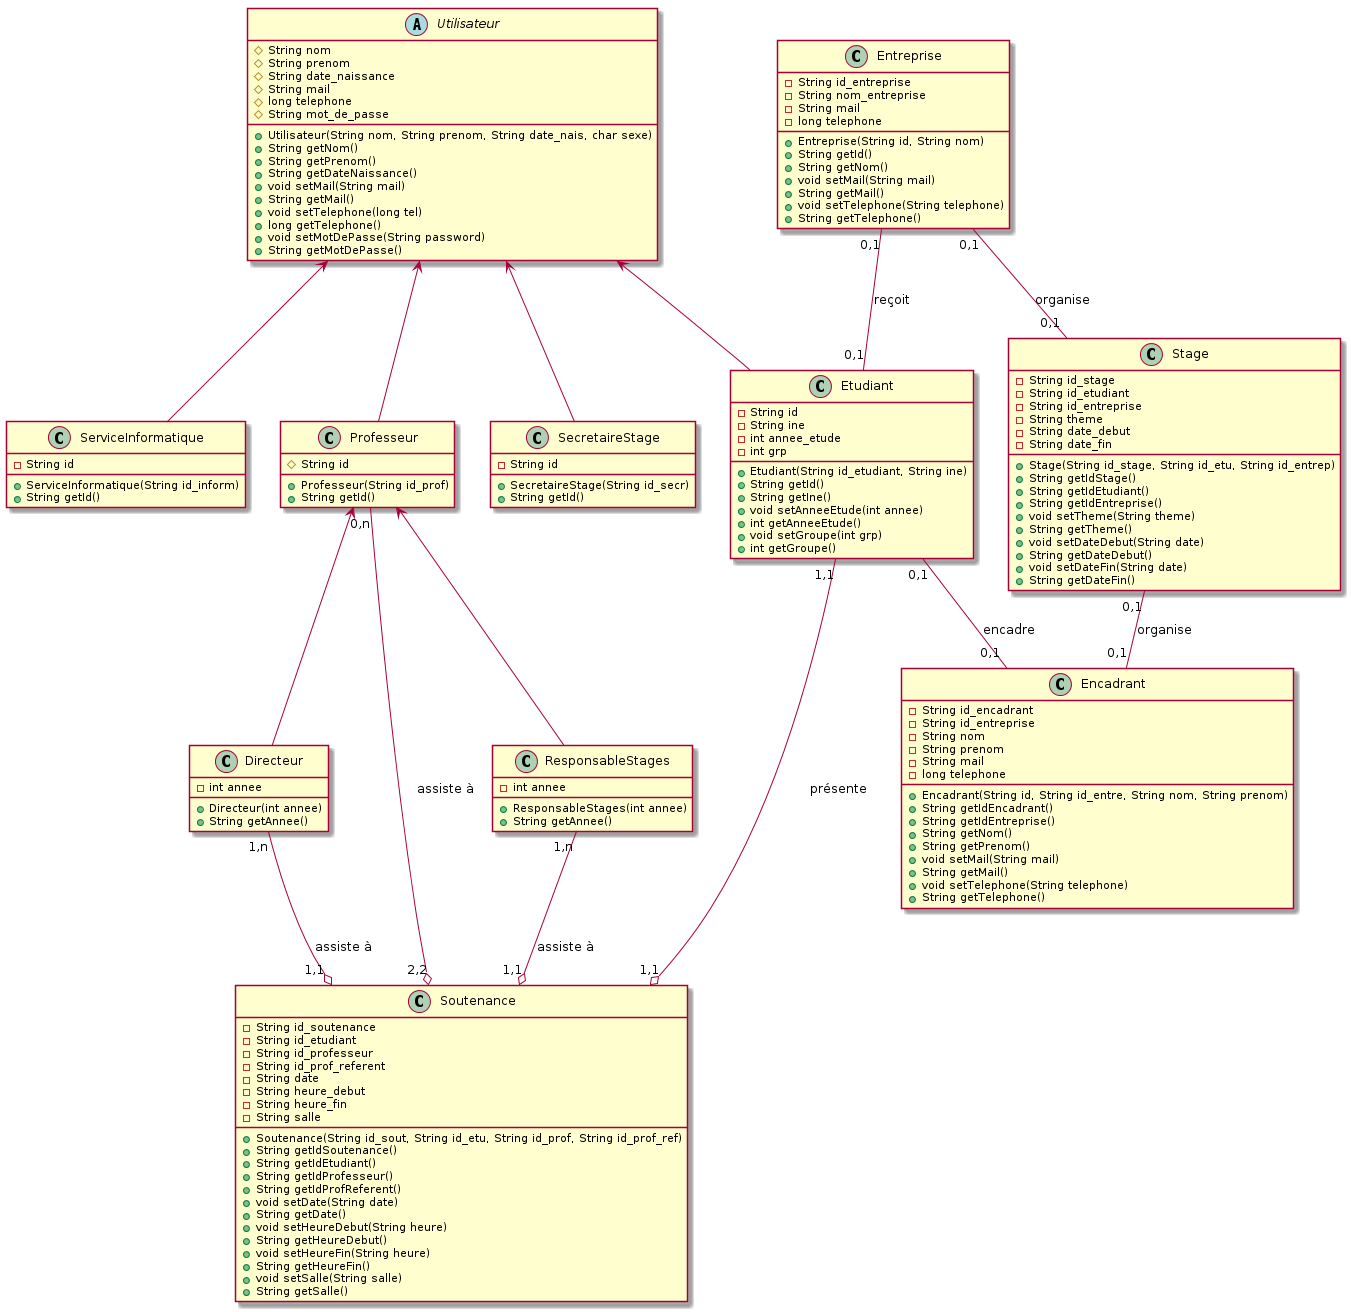
\includegraphics[scale=0.4]{Images/diagrammedesclasses.png}}
\hspace{1cm}Notre façon de représenter les données a un peu évolué depuis la création du diagramme entités-associations. Nous avons notamment pris en compte le rôle de l’entreprise et de l’encadrant dont les informations doivent être conservées, bien qu’ils n’utilisent pas l’application, de façon à pouvoir émettre la convention de stage.\vspace{0.2cm}

\hspace{0.6cm}Pour simplifier l’implémentation et éviter la recopie de code, nous avons choisi de faire hériter les types d’utilisateurs d’une super classe Utilisateur qui rassemble les informations que ceux-ci ont tous en commun.\vspace{0.2cm}

\hspace{0.6cm}Ce diagramme des classes représente par ailleurs les liens entre les différentes classes. Par exemple, il expose les types d’utilisateurs assistant à la soutenance et en quel nombre. Les liens entre l’entreprise, l’encadrant et le stage y sont aussi représentés.\\

\let\clearpage

\chapter*{Diagrammes de séquence}

\section*{Saisie de la fiche de renseignements}
\centerline{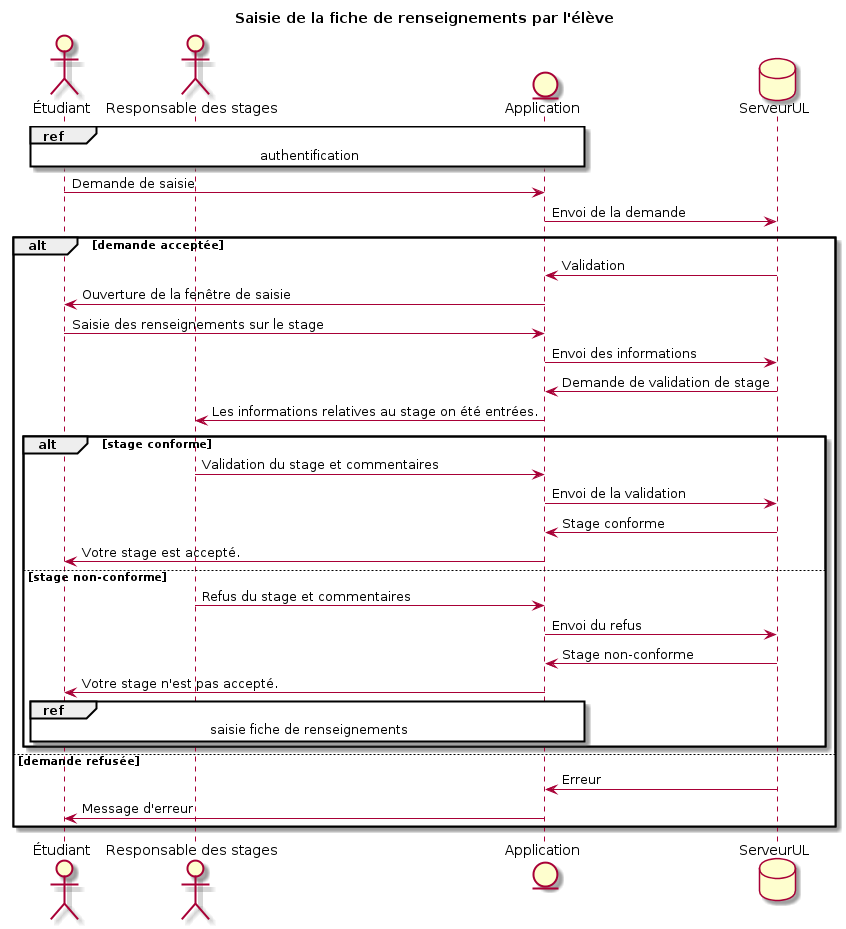
\includegraphics[scale=0.55]{Images/saisieficherenseignements.png}}
\hspace{1cm}Ce premier diagramme de séquence décrit la saisie de la fiche de renseignements par l’élève après qu’il a trouvé un stage.\vspace{0.2cm}

\hspace{0.6cm}Après s’être identifié, il entre les différentes informations dans les champs correspondant sur la page de saisie. Une fois cette opération terminée, les informations sont envoyées au serveur qui les transfère au responsable des stages pour validation. \vspace{0.2cm}

\hspace{0.6cm}Si le stage n’est pas conforme à ce qui est attendu, l’élève doit en trouver un autre et est invité à remplir une nouvelle fois la fiche de renseignements.

\section*{Prise de décision concernant une fiche de renseignements}
\centerline{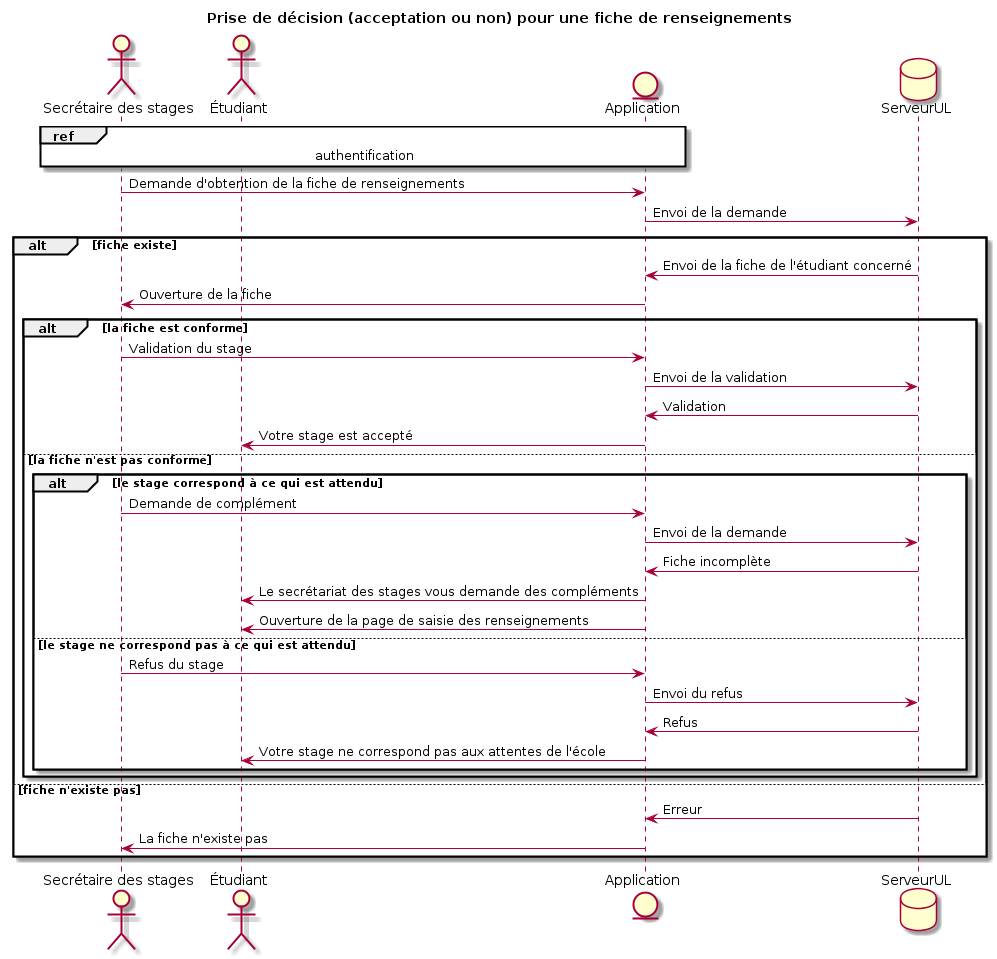
\includegraphics[scale=0.5]{Images/prisededecisionfichederenseignements.png}}
\hspace{1cm}Ce diagramme de séquence modélise la prise de décision concernant la fiche de renseignements une fois que l’élève l’a saisie et envoyée. C’est la secrétaire des stages qui prend cette décision.\vspace{0.2cm}

\hspace{0.6cm}La secrétaire des stages doit tout d’abord s’identifier. Elle envoie ensuite une demande d’obtention de la fiche de renseignements (associée à un étudiant) au serveur de l’Université de Lorraine via l’application. \vspace{0.2cm}

\hspace{0.6cm}Si la fiche existe et qu’elle est conforme, elle doit accepter le stage. Si la fiche est incomplète mais que le stage correspond aux attentes de l’école, alors une demande de compléments est envoyée à l’étudiant concerné, puis la fiche est de nouveau étudiée par la secrétaire des stages. Si la fiche ne correspond pas aux attentes de l’école, le stage est refusé. Si la fiche n’existe pas, aucune décision n’est prise (dans le délai renseigné par la secrétaire). \vspace{0.2cm}

\hspace{0.6cm}Chaque étudiant aura besoin de s’identifier pour consulter la décision. 
 
\section*{Initialisation d'une nouvelle année}
\centerline{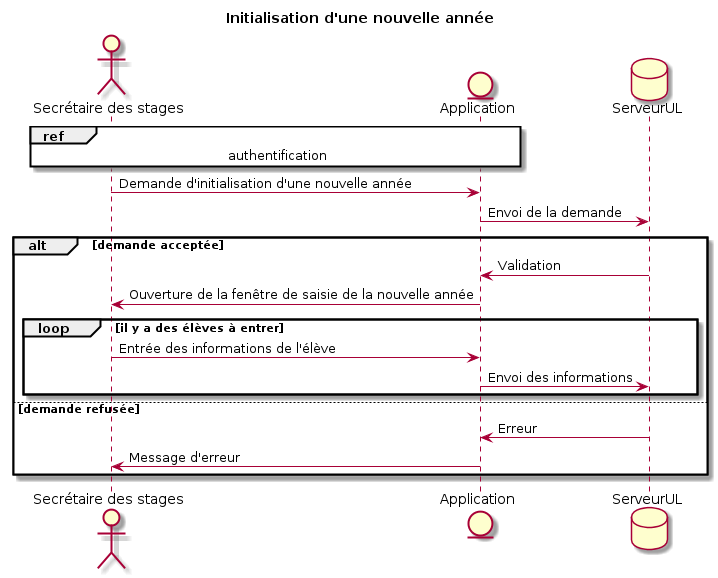
\includegraphics[scale=0.6]{Images/initialisationnouvelleannee.png}}
\hspace{1cm}Le dernier diagramme de séquence que nous avons été amenés à réaliser décrit l’initialisation d’une nouvelle année par le secrétaire des stages.\vspace{0.2cm}

\hspace{0.6cm}Celui-ci commence par s’identifier. Il envoie ensuite une requête au serveur par le biais de l’application pour pouvoir entrer les informations des élèves de la nouvelle année. Une fois la fenêtre de saisie ouverte, il peut entrer les informations nécessaires pour chaque étudiant.\vspace{0.2cm}

\hspace{0.6cm}Par ailleurs, l’application augmente automatiquement d’un la valeur de l’année de tous les élèves déjà enregistrés à l’initialisation d’une nouvelle année par le secrétaire des stages.

\newpage

\chapter*{Diagramme d'états}
\centerline{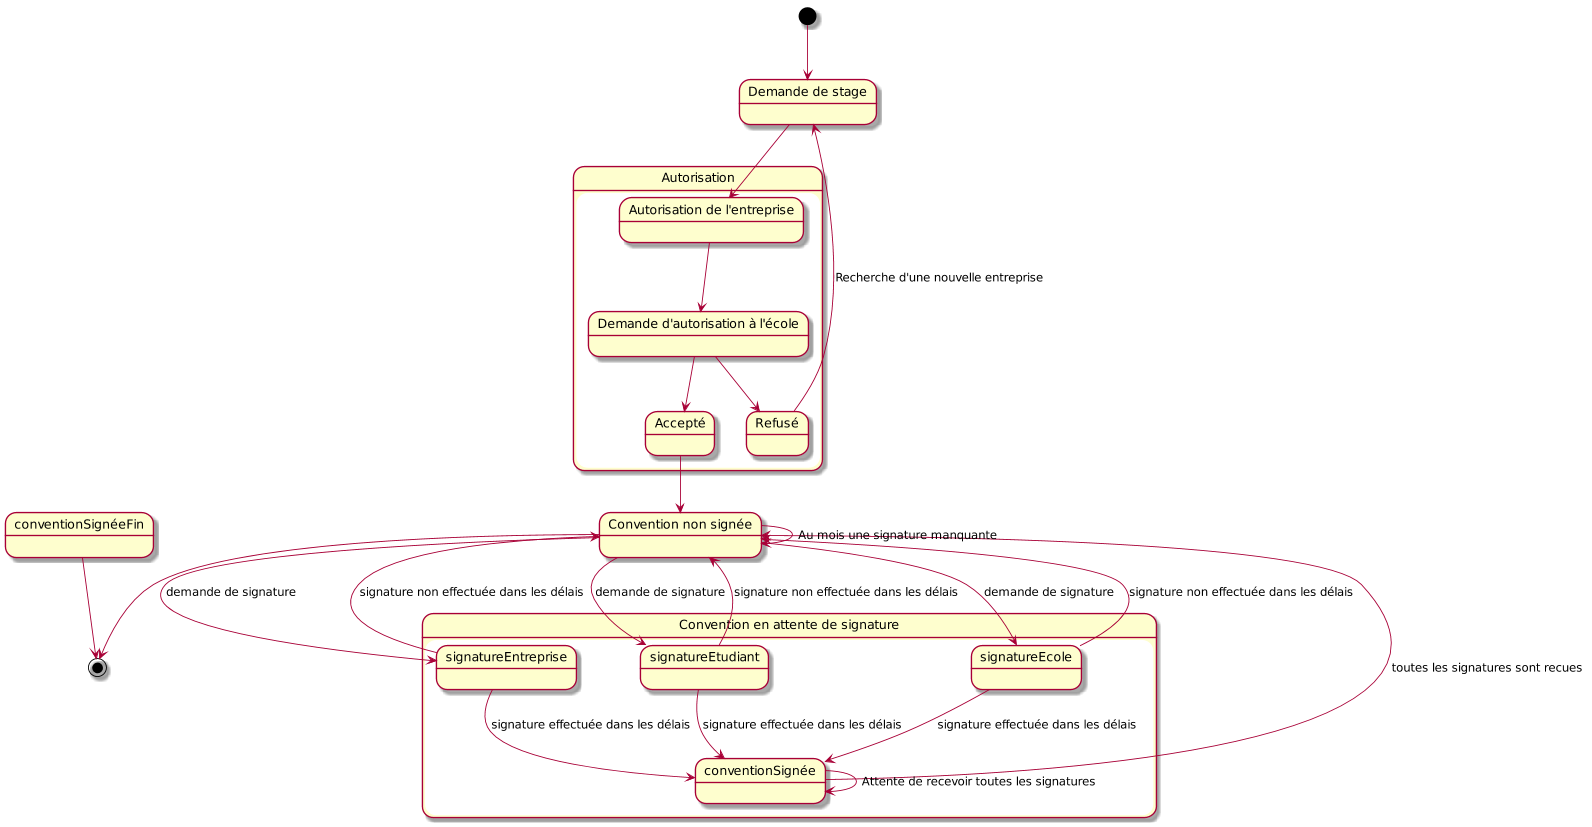
\includegraphics[scale=0.35]{Images/diagrammedetats.png}}
\hspace{1cm}Ce diagramme d’états correspond à une demande de stage. Il décrit la situation de la validation ou non du stage depuis le moment de la demande à l’entreprise jusqu’à la signature par les trois partis.\vspace{0.2cm}

\hspace{0.6cm}L’état initial de la demande à l’entreprise est validé si l’élève obtient l’autorisation de rejoindre la société pour son stage. Dans ce cas, l’école doit aussi donner son accord et s’assurer que le stage est conforme à ce qui est attendu. Sinon, l’élève se doit de trouver un autre stage.\vspace{0.2cm}

\hspace{0.6cm}Si l’école accepte le stage, la convention est émise et on est en attente de signature des trois parties. Pour que le stage ait finalement lieu, il est nécessaire que les trois partis rendent la convention signée dans les temps.

\newpage

\appendix
\chapter*{Annexe A : Diagramme entités-associations}
\begin{center}
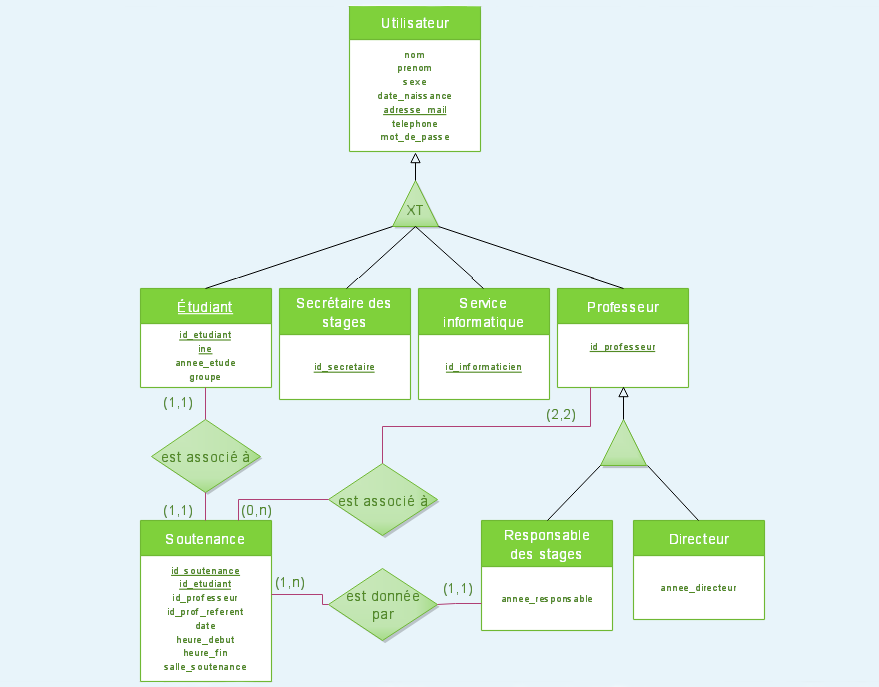
\includegraphics[scale=0.5]{Images/diagentiassoc.png}
\end{center}

\newpage

\chapter*{Annexe B : Code UML des diagrammes}

\section*{Diagramme des classes}
\begin{verbatim}
@startuml

abstract class Utilisateur {
	#String nom
	#String prenom
	#String date_naissance
	#String mail
	#long telephone
	#String mot_de_passe
	+Utilisateur(String nom, String prenom, String date_nais, char sexe)
	+String getNom()
	+String getPrenom()
	+String getDateNaissance()
	+void setMail(String mail)
	+String getMail()
	+void setTelephone(long tel)
	+long getTelephone()
	+void setMotDePasse(String password)
	+String getMotDePasse()
}

class Etudiant {
	-String id
	-String ine
	-int annee_etude
	-int grp
	+Etudiant(String id_etudiant, String ine)
	+String getId()
	+String getIne()
	+void setAnneeEtude(int annee)
	+int getAnneeEtude()
	+void setGroupe(int grp)
	+int getGroupe()
}

class SecretaireStage {
	-String id
	+SecretaireStage(String id_secr)
	+String getId()
}

class ServiceInformatique {
	-String id
	+ServiceInformatique(String id_inform)
	+String getId()
}

class Professeur {
	#String id
	+Professeur(String id_prof)
	+String getId()
}

class ResponsableStages {
	-int annee
	+ResponsableStages(int annee)
	+String getAnnee()
}

class Directeur {
	-int annee
	+Directeur(int annee)
	+String getAnnee()
}

class Soutenance {
	-String id_soutenance
	-String id_etudiant
	-String id_professeur
	-String id_prof_referent
	-String date
	-String heure_debut
	-String heure_fin
	-String salle
	+Soutenance(String id_sout, String id_etu, String id_prof, String id_prof_ref)
	+String getIdSoutenance()
	+String getIdEtudiant()
	+String getIdProfesseur()
	+String getIdProfReferent()
	+void setDate(String date)
	+String getDate()
	+void setHeureDebut(String heure)
	+String getHeureDebut()
	+void setHeureFin(String heure)
	+String getHeureFin()
	+void setSalle(String salle)
	+String getSalle()
}

class Stage {
	-String id_stage
	-String id_etudiant
	-String id_entreprise
	-String theme
	-String date_debut
	-String date_fin
	+Stage(String id_stage, String id_etu, String id_entrep)
	+String getIdStage()
	+String getIdEtudiant()
	+String getIdEntreprise()
	+void setTheme(String theme)
	+String getTheme()
	+void setDateDebut(String date)
	+String getDateDebut()
	+void setDateFin(String date)
	+String getDateFin()
}

class Entreprise {
	-String id_entreprise
	-String nom_entreprise
	-String mail
	-long telephone
	+Entreprise(String id, String nom)
	+String getId()
	+String getNom()
	+void setMail(String mail)
	+String getMail()
	+void setTelephone(String telephone)
	+String getTelephone()
}

class Encadrant {
	-String id_encadrant
	-String id_entreprise
	-String nom
	-String prenom
	-String mail
	-long telephone
	+Encadrant(String id, String id_entre, String nom, String prenom)
	+String getIdEncadrant()
	+String getIdEntreprise()
	+String getNom()
	+String getPrenom()
	+void setMail(String mail)
	+String getMail()
	+void setTelephone(String telephone)
	+String getTelephone()
}

Utilisateur <-- Etudiant
Utilisateur <-- SecretaireStage
Utilisateur <-- ServiceInformatique
Utilisateur <-- Professeur
Professeur <-- ResponsableStages
Professeur <-- Directeur
Etudiant "1,1" --o "1,1" Soutenance : présente
Professeur "0,n" --o "2,2" Soutenance : assiste à
ResponsableStages "1,n" --o "1,1" Soutenance : assiste à
Directeur "1,n" --o "1,1" Soutenance : assiste à
Etudiant "0,1" -- "0,1" Encadrant : encadre
Stage "0,1" -- "0,1" Encadrant : organise
Entreprise "0,1" -- "0,1" Stage : organise
Entreprise "0,1" -- "0,1" Etudiant : reçoit

@enduml
\end{verbatim}


\section*{Saisie de la fiche de renseignements}
\begin{verbatim}
@startuml

title Saisie de la fiche de renseignements par l'élève

actor Étudiant
actor "Responsable des stages"
entity Application
database ServeurUL

ref over Étudiant, Application : authentification

Étudiant -> Application : Demande de saisie
Application -> ServeurUL : Envoi de la demande 

alt demande acceptée
	ServeurUL -> Application : Validation
	Application -> Étudiant : Ouverture de la fenêtre de saisie
	'Étudiant -> Application : Saisie du lieu du stage
	'Application -> ServeurUL : Envoi des informations
	'Étudiant -> Application : Saisie du service accueillant l'élève
	'Application -> ServeurUL : Envoi des informations
	'Étudiant -> Application : Saisie des informations concernant le stage
	'Application -> ServeurUL : Envoi des informations
	Étudiant -> Application : Saisie des renseignements sur le stage
	Application -> ServeurUL : Envoi des informations
	ServeurUL -> Application : Demande de validation de stage
	Application -> "Responsable des stages" : Les informations relatives au stage on été entrées.
	alt stage conforme
		"Responsable des stages" -> Application : Validation du stage et commentaires
		Application -> ServeurUL : Envoi de la validation
		ServeurUL -> Application : Stage conforme
		Application -> Étudiant : Votre stage est accepté.
	else stage non-conforme
		"Responsable des stages" -> Application : Refus du stage et commentaires
		Application -> ServeurUL : Envoi du refus
		ServeurUL -> Application : Stage non-conforme
		Application -> Étudiant : Votre stage n'est pas accepté.
		ref over Étudiant, Application : saisie fiche de renseignements
	end
else demande refusée
	ServeurUL -> Application : Erreur
	Application -> Étudiant : Message d'erreur
end
@enduml
\end{verbatim}


\section*{Prise de décision concernant une fiche de renseignements}
\begin{verbatim}
@startuml

title Prise de décision (acceptation ou non) pour une fiche de renseignements

actor "Secrétaire des stages"
actor Étudiant
entity Application
database ServeurUL

ref over "Secrétaire des stages", Application : authentification

"Secrétaire des stages" -> Application : Demande d'obtention de la fiche de renseignements
Application -> ServeurUL : Envoi de la demande 

alt fiche existe
	ServeurUL -> Application : Envoi de la fiche de l'étudiant concerné
	Application -> "Secrétaire des stages" : Ouverture de la fiche
	alt la fiche est conforme
		"Secrétaire des stages" -> Application : Validation du stage
		Application -> ServeurUL : Envoi de la validation
		ServeurUL -> Application : Validation
		Application -> Étudiant : Votre stage est accepté
	else la fiche n'est pas conforme
		alt le stage correspond à ce qui est attendu
			"Secrétaire des stages" -> Application : Demande de complément
			Application -> ServeurUL : Envoi de la demande
			ServeurUL -> Application : Fiche incomplète
			Application -> Étudiant : Le secrétariat des stages vous demande des compléments
			Application -> Étudiant : Ouverture de la page de saisie des renseignements
		else le stage ne correspond pas à ce qui est attendu
			"Secrétaire des stages" -> Application : Refus du stage
			Application -> ServeurUL : Envoi du refus
			ServeurUL -> Application : Refus
			Application -> Étudiant : Votre stage ne correspond pas aux attentes de l'école
		end
	end
else fiche n'existe pas
	ServeurUL -> Application : Erreur
	Application -> "Secrétaire des stages" : La fiche n'existe pas
end
@enduml
\end{verbatim}


\section*{Initialisation d'une nouvelle année}
\begin{verbatim}
@startuml

title Initialisation d'une nouvelle année

actor "Secrétaire des stages"
entity Application
database ServeurUL

ref over "Secrétaire des stages", Application : authentification

"Secrétaire des stages" -> Application : Demande d'initialisation d'une nouvelle année
Application -> ServeurUL : Envoi de la demande 

alt demande acceptée
	ServeurUL -> Application : Validation
	Application -> "Secrétaire des stages" : Ouverture de la fenêtre de saisie de la nouvelle année
	loop il y a des élèves à entrer
		"Secrétaire des stages" -> Application : Entrée des informations de l'élève
		Application -> ServeurUL : Envoi des informations
	end
else demande refusée
	ServeurUL -> Application : Erreur
	Application -> "Secrétaire des stages" : Message d'erreur
end

@enduml
\end{verbatim}


\section*{Diagramme d'états}
\begin{verbatim}
@startuml

scale 1600 width
state "Demande de stage" as dds
[*] --> dds

state Autorisation {
	state "Autorisation de l'entreprise" as autEnt
	state "Demande d'autorisation à l'école" as autEc
	dds -down-> autEnt
	autEnt -down-> autEc
	autEc -down-> Accepté
	autEc -down-> Refusé
}

state "Convention non signée" as convNnSignee
Refusé -up-> dds : recherche d'une nouvelle entreprise
Accepté -down-> convNnSignee

state "Convention en attente de signature" as convAttSign {
	state "Convention non signée" as nonSignee
	state "Signature de l'entreprise" as signatureEntreprise
	state "Signature de l'école" as signatureEcole
	state "Signature de l'étudiant" as signatureEtudiant
	state "Convention signée" as conventionSignée

	convNnSignee -> signatureEntreprise
	convNnSignee -> signatureEcole
	convNnSignee -> signatureEtudiant
	signatureEntreprise -down-> conventionSignée : dans les délais
	signatureEcole -down-> conventionSignée : dans les délais
	signatureEtudiant -down-> conventionSignée : dans les délais
	signatureEntreprise -down-> nonSignee : pas à temps
	signatureEcole -down-> nonSignee : pas à temps
	signatureEtudiant -down-> nonSignee : pas à temps

	conventionSignée->conventionSignée : attente de toutes les signatures
	nonSignee->convNnSignee
}

convNnSignee -up-> dds : recherche d'une nouvelle entreprise
conventionSignée -down->[*] : toutes les signatures sont reçues 

@enduml
\end{verbatim}

\newpage


\end{document}